\documentclass[11pt]{article}
\usepackage[margin=3cm]{geometry}
\usepackage{geometry} % Change margins if necessery here
\usepackage[swedish]{babel}
\usepackage[utf8]{inputenc}
\usepackage[T1]{fontenc}
\usepackage{fancyhdr}
\usepackage{ragged2e}
\usepackage{titling} % Make custom titles.
\usepackage{graphicx} % Allow graphics.
\usepackage{pbox} % Used for margins in tables.
\usepackage{tabularx} % Used for tables.
\usepackage{longtable} % Used for tables.
\usepackage{tabu} % Used for tables.
\usepackage{url} % Allow urls.
\usepackage{amsmath} % Allow math \begin{equation}, end
\usepackage[backend=biber,style=ieee]{biblatex} % Bibliography package. Bibtex/Biber depending on compilator
\usepackage{csquotes} % Spawns an error if not included. Not sure why.
\usepackage[hidelinks]{hyperref} % To include urls, hyper links and clickable references
\usepackage[nottoc]{tocbibind} % To include bibliography in ToC
\usepackage{comment} %allows comment
\usepackage{capt-of}
\usepackage{cases}
\usepackage{listings}
\usepackage{color}
\usepackage[normalem]{ulem}
\usepackage{tikz}
\usepackage{PTSansNarrow}
\usepackage{subcaption}
\usepackage{float}
\usepackage{todonotes} % Allows todos
\usepackage{placeins} %FloatBarrier
\date{\today} % Sets date to blank. Use \today to print todays date.
\usepackage{pdfpages} %Allows includepdf-command
\usepackage[font=it]{caption} % Sets capotions to italic
\usepackage[]{algorithm2e}
\usepackage{parskip} % Makes indenting of new paragraphs with new line and not tab
\usepackage{menukeys}

\graphicspath{ {images/} }
\newcommand{\subtitle}[1]{%
  \posttitle{%
    \par\end{center}
    \begin{center}\large#1\end{center}
    \vskip0.5em}%
}
\pagestyle{fancy}


\date{\today}
\pagenumbering{roman}
\chead{Användarmanual - resQ.PL}
\rhead{\today}
\lhead{}
\lfoot{
	TSEA56
 \\
    Användarmanual resQ.PL
}
\rfoot{
	Projektgrupp 2
	\\
	e-post: adnbe196@student.liu.se
}

\addbibresource{refs.bib} 

\begin{document}
\begin{titlepage}
\begin{center}
{{\Large\bfseries Användarmanual resQ.PL} \\ Kandidatprojekt i elektronik vid Linköpings Universitet}\\
%
\vspace{1\baselineskip}
%
Version 0.1\\
\vspace{2\baselineskip}

\vspace{2\baselineskip}
\today

\end{center}
\end{titlepage}

\pagebreak
\begin{center}

\section*{PROJEKTIDENTITET}
2015/VT, Undsättningsrobot Gr. 2
\\
Linköpings tekniska högskola, ISY
\\[0.5in]
\begin{table}[h]
\begin{tabular}{|l|p{0.3\linewidth}|l|l|} \hline
Namn & Ansvar & Telefon & E-post \\[0.1in] \hline
Nikolaj Agafonov & Dokumentansvarig (DA) & 072-276 99 46 & nikag669@student.liu.se \\ \hline
Adnan Berberovic & Projektledare (PL) & 070-491 96 07 & adnbe196@student.liu.se \\ \hline
Andreas Brorsson & Testansvarig (TA) & 073-524 44 60 & andbr981@student.liu.se \\ \hline
Fredrik Fridborn & Designansvarig Sensormo-
dul (DSE) & 073-585 52 01 & frefr166@student.liu.se \\ \hline
Robert Oprea & Designansvarig Styrmodul (DST) & 070-022 10 18 & robop806@student.liu.se \\ \hline
Måns Skytt & Designansvarig Kommunikationsmodul (DK) & 070-354 28 84 & mansk700@student.liu.se \\ \hline
\end{tabular}
\end{table}

E-postlista för hela gruppen: adnbe196@student.liu.se
\\[1in]
Kund: Kent Palmkvist, 581 83 Linköping,
Kundtelefon: 013-28 13 47, kentp@isy.liu.se
\\[1in]
Kursansvarig: Tomas Svensson, 013-28 13 68, tomass@isy.liu.se
\\
Handledare: Olov Andersson, 013-28 26 58, Olov.Andersson@liu.se
\end{center}
\pagebreak

\tableofcontents

\pagebreak

\section*{Dokumenthistorik}
\begin{table}[h]
\begin{tabular}{|l|l|l|l|l|} \hline

Version & 
Datum & 
Utförda förändringar & 
Utförda av & 
Granskad \\[0.1in] \hline
0.1 &
\today & 
Första utkastet & 
ABr & 
- \\ \hline


\end{tabular}
\end{table}


\pagebreak

\pagenumbering{arabic}


% ***** RAPPORTDELEN *****
\section{Inledning}
Denna användarmanual redogör hur undsättningsroboten resQ.PL används. Den första sektionen beskriver hur en besiktning av roboten före användning sker. Besiktningen säkerställer att kablar,sensorer och strömförsörjning sitter rätt.  I den andra sektionen redogörs hur robotens används i det manuella respektive autonoma läget. 

\pagebreak    


\section{Före användning av robot}
För att nyttja roboten krävs först att roboten är i sådant skick att den kan startas. Med en okulär besiktning kontolleras att nedan listad hårdvara finns och är rätt kopplad, mer utförlig förklaring ges i användarmanualen, se appendix~\ref{appendix:användarmanual}. 


\begin{itemize}
\item Strömbrytaren i bak på robotens chassi är avslagen under hela besikting och när kablar kopplas.
\item Batteri med 7.2V spänning inkopplat. 
\item 16-pin flatkabel mellan styrmodulen och sensormodulen är inkopplad.
\item 10-pin flatkabel mellan robotens chassi och styrmodulen är inkopplad.
\item Reflexsensorn för avståndsmätning är kopplad till styrmodulen.
\item Gripklon är kopplad till styrmodulen.
\item Övriga sensorers kablar är kopplade till sensormodulen.
\item Blåtands-modemet är anslutet.
\item Brytaren för autonomt eller manuellt läge slås över till manuellt läge initial.
\end{itemize}

\subsection{Kalibrering}  
På grund av att robotens underlag och omgivning varierar medför miljöbyte att sensorernas resultat avviker vid samma mätningar. Därför bör sensorerna kalibreras varje gång miljön roboten befinner sig i ändras. Om roboten inte kalibreras finns det en risk att roboten t.ex. inte känner av mållinje-tejpen vilket gör att uppdraget aldrig slutförs. Kalibreringen utförs genom att placera roboten på marken så att reflexsensorn i fronten inte befinner sig över den svarta målgångs-tejpen, roboten står i startposition med vägg på var sida. När roboten är placerad i startposition trycks den ?SVARTA/RÖDA? brytaren på sensormodulen för kalibrering. 

\section{Användning av robot}
Roboten har två arbetslägen, autonom och manuellt läge. När strömmen slås på med brytaren i bak på chassit bör brytaren som väljer läge vara inställd på manuellt läge för att roboten inte ska röra sig. När strömmen slås på lyser LCD-skärmen upp med meddelandet: ”MANUAL MODE”.


\pagebreak

\subsection{Manuellt läge}
I manuellt läge krävs en Windows-dator men blåtand och programvaran som utvecklats till roboten. Brytaren på roboten sätts till manuellt läge och programvaran startas. Figur~\ref{fig:man} nedan visar gränssnittet i manuellt läge. Roboten skickar ut information från sensorer och position i labyrinten som syns i nedre hörnet till vänster i det grafiska gränssnittet, dessa värden uppdateras kontinuerligt. 


\begin{figure}[H]
\begin{center}
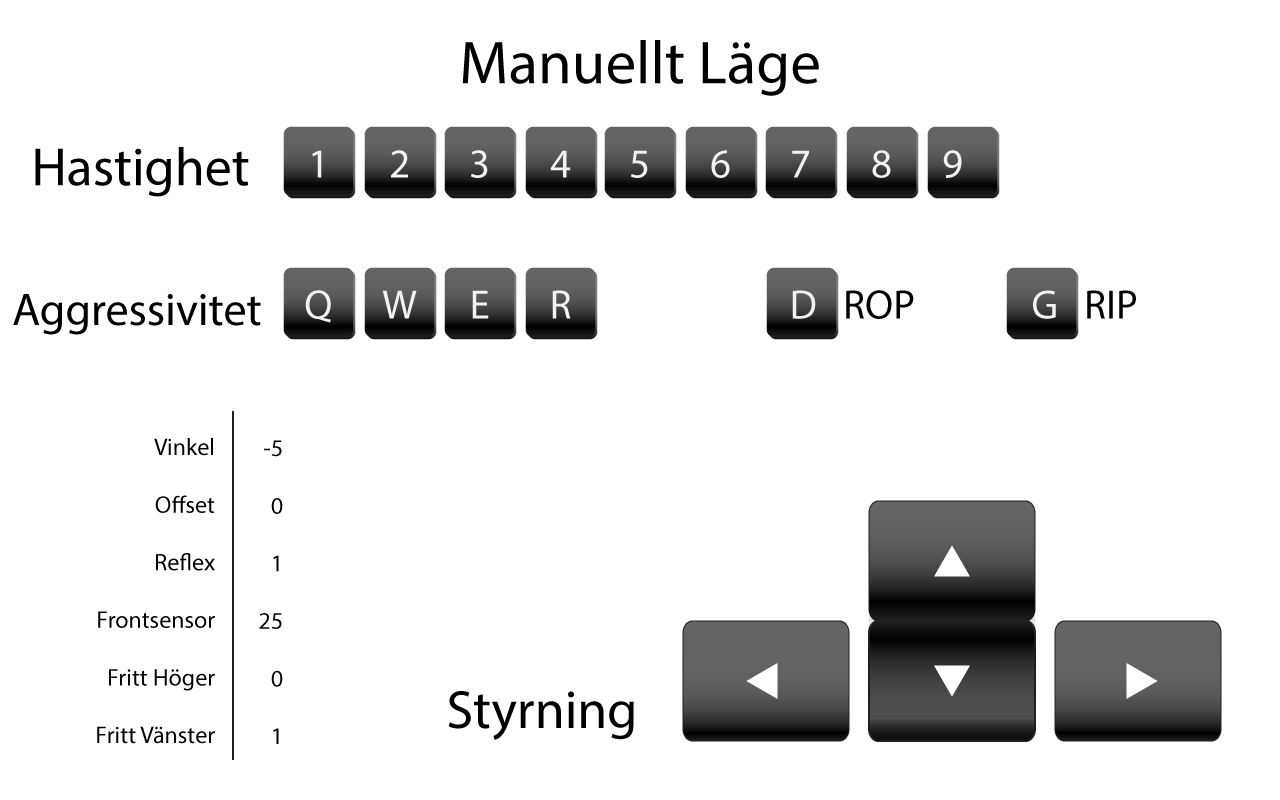
\includegraphics[scale=0.3]{Manual.png}
\caption{Manuell styrnings grafiska användargränssnitt}
\label{fig:man}
\end{center}
\end{figure}

Roboten styrs och regleras med tangenterna på datorn. De olika tangenterna och deras uppgift tabuleras i tabell \ref{tab:man}. 

\begin{table}[H]
\begin{center}

\begin{tabular}{|p{4cm}|p{10cm}|} \hline

\textbf{Tangent} & \textbf{Utför} \\ \hline

\keys{\arrowkeyup} & Roboten rörs framåt med vald hastighet, samma kraft på båda motorer. \\ \hline

\keys{\arrowkeydown} & Roboten rör sig bakåt med vald hastighet, samma kraft på båda motorer. \\ \hline

\keys{\arrowkeyright} & Roboten roterar medurs. \\ \hline

\keys{\arrowkeyleft}& Roboten roterar moturs. \\ \hline

\keys{\arrowkeyup + \arrowkeyright}& Roboten rörs framåt och svänger åt höger med vald aggressivitet och hastighet. \\ \hline

\keys{\arrowkeyup + \arrowkeyleft} & Roboten rörs framåt och svänger åt vänster med vald aggressivitet och hastighet. \\ \hline

\keys{\arrowkeydown + \arrowkeyright} & Roboten rörs bakåt och svänger åt höger med vald aggressivitet och hastighet. \\ \hline

\keys{\arrowkeydown + \arrowkeyleft} & Roboten rörs bakåt och svänger åt vänster med vald aggressivitet och hastighet. \\ \hline


\keys{G} &  Öppnar gripklon. \\ \hline

\keys{D} &  Stänger gripklon. \\ \hline

\keys{Q}, \keys{ W}, \keys{E}, \keys{R} &  Styr med vilken agressivitet roboten ska svänga med, från att svänga runt sin egen axel till att svänga en viss grad.  \\ \hline

\keys{1}, \keys{2}, \keys{3}, \keys{4}, \keys{5}, \keys{6}, \keys{7}, \keys{8}, \keys{9} &  Styr hastigheten på roboten med vald  kraft till motorerna.  \\ \hline

\end{tabular}
\caption{Manuella lägets tangentstyrning}
\label{tab:man}
\end{center}
\end{table}

\subsection{Autonomt läge}
I det autonoma läget ska roboten befinna sig i en labyrint enligt tävlingsreglerna se appendix~\ref{appendix:regler}. Roboten ställs mellan två väggar centrerat vinkelrätt i början på labyrinten i så kallad startposition. Brytaren för vilket läge roboten ska vara i ställs till autonom. Roboten kommer då att utforska labyrinten, hitta målet och sedan åka tillbaka till startpositionen.





%Might have to compile TWICE.
\printbibliography 

\pagebreak	

%\input{chapters/appendix}   %Vid inlämning, kommentera bort.


	



\end{document}
